\documentclass[conference]{IEEEtran}

\usepackage{amsmath,amssymb,amsfonts}
\usepackage{graphicx}
\usepackage{textcomp}
\usepackage{booktabs}
\usepackage{multirow}
\usepackage{xcolor}
\usepackage{hyperref}
\usepackage{float}
\usepackage{array}
\usepackage{tabularx}
\usepackage{caption}
\usepackage{subcaption}
\usepackage{tikz}
\usetikzlibrary{positioning, arrows.meta, shapes.geometric, fit, backgrounds, calc, decorations.pathreplacing}

\hypersetup{
    colorlinks=true,
    linkcolor=blue,
    citecolor=blue,
    urlcolor=blue
}

\begin{document}

\title{Kenya Sign Language Recognition Using Temporal Graph Convolutional Networks with Signer-Invariant Feature Learning}

\author{
\IEEEauthorblockN{Hassan Mahmoud}
\IEEEauthorblockA{
University of Colorado Boulder\\
Boulder, CO, USA\\
hama5612@colorado.edu}
}

\maketitle

% ============================================================
% ABSTRACT
% ============================================================
\begin{abstract}
Sign language recognition for under-resourced languages is hard---harder than most benchmark papers would have you believe. We present the first automated recognition system for Kenya Sign Language (KSL), covering 30 sign classes: 15 numbers and 15 common words. The system extracts hand and upper-body landmarks via MediaPipe Holistic, builds a 48-node skeleton graph, and classifies signs with a Spatial-Temporal Graph Convolutional Network (ST-GCN) paired with a Gradient Reversal Layer (GRL) for signer-invariant feature learning. Over seven model iterations (v19--v25), we tried just about everything the literature recommends: multi-stream fusion, prototypical classification, MixStyle domain randomization, ArcFace angular margin loss, hand-to-body spatial features, temporal CutMix, and a battery of data augmentation strategies. Our best model hits 93.3\% validation accuracy with just 776K parameters, but real-world evaluation on three unseen signers tells a different story---combined accuracy tops out at 40.7\%. We also ran leave-one-signer-out cross-validation, which gave us 94.7\% but still predicted real-world performance poorly (a 56-point gap). The honest finding: four training signers impose a hard ceiling on cross-signer generalization that no amount of architectural cleverness can break through. These results offer practical guidance for anyone building skeleton-based sign language recognition systems in low-resource settings.
\end{abstract}

\begin{IEEEkeywords}
Kenya Sign Language, graph convolutional networks, sign language recognition, domain generalization, MediaPipe, signer invariance
\end{IEEEkeywords}

% ============================================================
% 1. INTRODUCTION
% ============================================================
\section{Introduction}

Roughly 600,000 deaf and hard-of-hearing Kenyans depend on Kenya Sign Language (KSL) as their primary means of communication~\cite{ai4ksl2024}. KSL gained official recognition in Kenya's 2010 Constitution, yet from a computational standpoint it remains almost entirely neglected. Automated recognition systems exist for ASL, CSL, BSL, and a growing number of other sign languages---but for KSL, there's essentially nothing. That gap matters. It means the Kenyan deaf community is locked out of the accessibility technologies that speakers of better-resourced sign languages increasingly take for granted.

The field of sign language recognition (SLR) has come a long way from the days of data gloves and depth cameras. Modern systems lean on pose estimation frameworks to pull out skeletal keypoints from ordinary video~\cite{robert2023review}, and landmark-based methods offer real advantages: they're more robust to lighting changes, cluttered backgrounds, and differences in signer appearance than raw RGB approaches~\cite{aiman2023}. Graph Convolutional Networks, first brought to skeleton-based action recognition by Yan et al.~\cite{yan2018stgcn}, have become the go-to tool for capturing how body joints relate to each other in space and time.

But there's a catch. Cross-signer generalization---getting a model trained on a handful of signers to work on people it's never seen---remains brutally difficult. It's the sign language equivalent of speaker-independent speech recognition, and it can be framed as a domain generalization problem where each signer is a separate domain~\cite{pu2024signer}. This problem gets worse, not better, when you're dealing with an under-resourced language where recruiting signers is itself a challenge.

This paper introduces the first automated KSL recognition system, targeting 30 sign classes (15 numbers and 15 common words). We use MediaPipe Holistic~\cite{zhang2020mediapipe} for landmark extraction and a temporal GCN with a Gradient Reversal Layer~\cite{ganin2016domain} to learn signer-invariant features. Across seven iterations, we systematically tested multi-stream fusion~\cite{shi2019twostreamAGCN}, prototypical classification~\cite{snell2017prototypical}, MixStyle domain randomization~\cite{zhou2021mixstyle}, ArcFace angular margin loss~\cite{deng2019arcface}, hand-to-body spatial features, temporal CutMix, and a wide array of skeleton-based augmentations~\cite{kolawole2024augmentation}.

Our key contributions are:
\begin{enumerate}
    \item The first automated KSL recognition system, establishing a benchmark for this under-resourced language.
    \item A compact ST-GCN architecture (776K parameters) with GRL-based signer-invariant feature learning that reaches 93.3\% validation accuracy.
    \item Comprehensive ablation studies across seven model versions showing that architectural innovations---multi-stream fusion, prototypical networks, MixStyle, hand-body features---provide diminishing returns when training data comes from only four signers.
    \item Leave-one-signer-out cross-validation results (94.7\%) alongside real-world testing (40.7\%), exposing a 56-point gap that standard evaluation protocols miss entirely.
    \item Empirical evidence of a hard ceiling near 40\% accuracy on unseen signers, and honest reporting of the roughly 53-point gap between validation and deployment performance.
\end{enumerate}

% ============================================================
% 2. RELATED WORK
% ============================================================
\section{Related Work}

\subsection{Sign Language Recognition}

The landscape of landmark-based SLR is broad and growing. Anithadevi et al.~\cite{anithadevi2025} built a MediaPipe-LSTM pipeline for 30 Indian Sign Language categories that reached 97\% accuracy. Moustafa et al.~\cite{moustafa2023} paired MediaPipe hand landmarks with CNNs for Arabic Sign Language, hitting 97.1\%. Hasan et al.~\cite{hasan2025} showed that multimodal late fusion could push Bangla Sign Language recognition to 94.71\% across 200 word classes from 16 signers. Impressive numbers, all of them---but most of these systems test on signers who also appeared during training, which makes a direct comparison with our cross-signer evaluation protocol tricky at best. Kamal et al.~\cite{kamal2024} tackled data scarcity in continuous SLR using adversarial autoencoders, a challenge that sits at the heart of our work too.

\subsection{Graph Convolutional Networks for Skeleton-Based Recognition}

Yan et al.~\cite{yan2018stgcn} were the first to apply GCNs to skeleton-based action recognition with ST-GCN. The idea was elegant: treat joints as graph nodes, connect them with spatial edges that follow body structure, and add temporal edges linking the same joint across frames. Shi et al.~\cite{shi2019twostreamAGCN} pushed this further with 2s-AGCN, which learns graph topology adaptively and combines joint and bone streams. Since then, Liu et al.~\cite{liu2020msg3d} introduced multi-scale aggregation (MS-G3D), Chen et al.~\cite{chen2021ctrgcn} added channel-wise topology refinement (CTR-GCN), and the field has kept moving. For hand gestures specifically, Aiman and Ahmad~\cite{aiman2023} found that angle-based features with GCN help combat overfitting on small datasets---a finding we can confirm. Our architecture builds on this ST-GCN lineage but adapts the graph topology for the 48-node skeleton that MediaPipe produces.

\subsection{Kenya Sign Language Research}

Published work on KSL recognition is, to put it plainly, almost nonexistent. The AI4KSL project~\cite{ai4ksl2024} created a digital open-access KSL dataset using MediaPipe---the closest prior work to what we're doing. Amukasa~\cite{amukasa2021} explored CNN-based KSL alphabet recognition. There's some related work on Ethiopian and Amharic sign languages, but those address different vocabularies and signing conventions. The scarcity of KSL-specific research is precisely why we felt this work was worth doing.

\subsection{Domain Generalization and Signer Independence}

Cross-signer generalization maps naturally onto domain generalization, where each signer is a distinct domain. Ganin et al.~\cite{ganin2016domain} gave us the Gradient Reversal Layer: during forward propagation it does nothing, but during backpropagation it flips the gradients, pushing the feature extractor to drop domain-specific (i.e., signer-specific) information. Pu et al.~\cite{pu2024signer} explicitly framed signer-independent SLR as domain generalization and showed gains from removing signer-specific features. Zhou et al.~\cite{zhou2021mixstyle} took a different angle with MixStyle, mixing feature statistics across domains at the instance level to hallucinate novel training domains without any extra parameters. We tried both approaches.

\subsection{Few-Shot Learning and Metric Learning}

Snell et al.~\cite{snell2017prototypical} introduced prototypical networks, classifying inputs by their distance to class centroids in embedding space. Guo et al.~\cite{guo2024fewshot} applied this to ASL on the WLASL dataset and got 43.75\% top-1---a number strikingly close to our own real-world results, which says something about the fundamental difficulty of sign recognition with limited data. Deng et al.~\cite{deng2019arcface} proposed ArcFace for learning discriminative embeddings through angular margin loss. We tried it. It didn't go well (more on that in Section~\ref{sec:arcface}).

\subsection{Multi-Stream Fusion}

Multi-stream architectures are standard practice in skeleton-based recognition. The recipe: train separate networks on different feature representations---joint positions, bone vectors, velocities---and fuse their predictions through late fusion~\cite{shi2019twostreamAGCN}. On big benchmarks like NTU RGB+D, this reliably helps. Whether it helps when you've got very few signers and you're testing on people the model has never seen is a different question, and one we answer directly.

% ============================================================
% 3. METHODS
% ============================================================
\section{Methods}

\subsection{Data Collection and Preprocessing}

\subsubsection{Video Collection}
We collected sign language videos from native KSL signers performing 30 isolated signs: 15 numbers (9, 17, 22, 35, 48, 54, 66, 73, 89, 91, 100, 125, 268, 388, 444) and 15 words (Agreement, Apple, Colour, Friend, Gift, Market, Monday, Picture, Proud, Sweater, Teach, Tomatoes, Tortoise, Twin, Ugali). Each signer recorded about 5 repetitions per sign. After deduplication, we ended up with roughly 250 training samples per category (numbers and words) from 4 unique signers.

\subsubsection{Landmark Extraction}
We run MediaPipe Holistic (v0.10.14) on every frame with model complexity 2, minimum detection confidence 0.5, and minimum tracking confidence 0.5. This gives us 549 dimensions per frame: 33 pose landmarks ($33 \times 3 = 99$ coordinates), 21 left-hand landmarks ($21 \times 3 = 63$), 21 right-hand landmarks ($21 \times 3 = 63$), 68 face keypoints ($68 \times 3 = 204$), and 40 lip detail points ($40 \times 3 = 120$).

\subsubsection{Node Selection and Graph Construction}
From those 549 features, we keep 48 nodes that matter for sign production: 21 left-hand joints, 21 right-hand joints, and 6 upper-body pose joints (shoulders, elbows, wrists). We discard face and lip landmarks since they don't contribute to the manual components of the signs in our vocabulary.

The skeleton graph $\mathcal{G} = (\mathcal{V}, \mathcal{E})$ has $|\mathcal{V}| = 48$ nodes linked by anatomical edges: 23 per hand following finger kinematic chains plus inter-finger connections, 7 pose edges connecting shoulders to elbows to wrists, and cross-body edges from wrists to hand roots. We also add a weak inter-hand edge (weight 0.3) between the left and right wrist nodes (Fig.~\ref{fig:skeleton}). The adjacency matrix gets symmetric normalization: $\hat{A} = D^{-1/2}(A + I)D^{-1/2}$.

\begin{figure}[t]
    \centering
    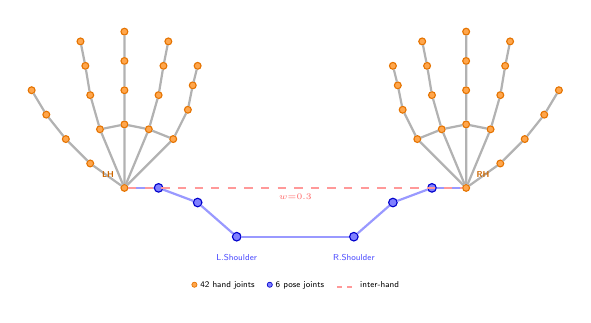
\begin{tikzpicture}[
        scale=0.62, transform shape,
        joint/.style={circle, fill=orange!70, draw=orange!90!black, inner sep=0pt, minimum size=4pt},
        pose/.style={circle, fill=blue!50, draw=blue!80!black, inner sep=0pt, minimum size=5pt},
        edge/.style={thick, gray!60},
        poseedge/.style={thick, blue!40},
        interhand/.style={thick, dashed, red!40},
    ]

    % === LEFT HAND (centered at 0,0) ===
    % Wrist
    \node[joint] (lw) at (-3.5, 0) {};

    % Thumb chain
    \node[joint] (l1) at (-4.2, 0.5) {};
    \node[joint] (l2) at (-4.7, 1.0) {};
    \node[joint] (l3) at (-5.1, 1.5) {};
    \node[joint] (l4) at (-5.4, 2.0) {};

    % Index chain
    \node[joint] (l5) at (-4.0, 1.2) {};
    \node[joint] (l6) at (-4.2, 1.9) {};
    \node[joint] (l7) at (-4.3, 2.5) {};
    \node[joint] (l8) at (-4.4, 3.0) {};

    % Middle chain
    \node[joint] (l9) at (-3.5, 1.3) {};
    \node[joint] (l10) at (-3.5, 2.0) {};
    \node[joint] (l11) at (-3.5, 2.6) {};
    \node[joint] (l12) at (-3.5, 3.2) {};

    % Ring chain
    \node[joint] (l13) at (-3.0, 1.2) {};
    \node[joint] (l14) at (-2.8, 1.9) {};
    \node[joint] (l15) at (-2.7, 2.5) {};
    \node[joint] (l16) at (-2.6, 3.0) {};

    % Pinky chain
    \node[joint] (l17) at (-2.5, 1.0) {};
    \node[joint] (l18) at (-2.2, 1.6) {};
    \node[joint] (l19) at (-2.1, 2.1) {};
    \node[joint] (l20) at (-2.0, 2.5) {};

    % Left hand edges
    \foreach \a/\b in {lw/l1, l1/l2, l2/l3, l3/l4, lw/l5, l5/l6, l6/l7, l7/l8, lw/l9, l9/l10, l10/l11, l11/l12, lw/l13, l13/l14, l14/l15, l15/l16, lw/l17, l17/l18, l18/l19, l19/l20, l5/l9, l9/l13, l13/l17}
        \draw[edge] (\a) -- (\b);

    % === RIGHT HAND (mirrored) ===
    \node[joint] (rw) at (3.5, 0) {};

    % Thumb
    \node[joint] (r1) at (4.2, 0.5) {};
    \node[joint] (r2) at (4.7, 1.0) {};
    \node[joint] (r3) at (5.1, 1.5) {};
    \node[joint] (r4) at (5.4, 2.0) {};

    % Index
    \node[joint] (r5) at (4.0, 1.2) {};
    \node[joint] (r6) at (4.2, 1.9) {};
    \node[joint] (r7) at (4.3, 2.5) {};
    \node[joint] (r8) at (4.4, 3.0) {};

    % Middle
    \node[joint] (r9) at (3.5, 1.3) {};
    \node[joint] (r10) at (3.5, 2.0) {};
    \node[joint] (r11) at (3.5, 2.6) {};
    \node[joint] (r12) at (3.5, 3.2) {};

    % Ring
    \node[joint] (r13) at (3.0, 1.2) {};
    \node[joint] (r14) at (2.8, 1.9) {};
    \node[joint] (r15) at (2.7, 2.5) {};
    \node[joint] (r16) at (2.6, 3.0) {};

    % Pinky
    \node[joint] (r17) at (2.5, 1.0) {};
    \node[joint] (r18) at (2.2, 1.6) {};
    \node[joint] (r19) at (2.1, 2.1) {};
    \node[joint] (r20) at (2.0, 2.5) {};

    % Right hand edges
    \foreach \a/\b in {rw/r1, r1/r2, r2/r3, r3/r4, rw/r5, r5/r6, r6/r7, r7/r8, rw/r9, r9/r10, r10/r11, r11/r12, rw/r13, r13/r14, r14/r15, r15/r16, rw/r17, r17/r18, r18/r19, r19/r20, r5/r9, r9/r13, r13/r17}
        \draw[edge] (\a) -- (\b);

    % === POSE (upper body) ===
    \node[pose] (ls) at (-1.2, -1.0) {};  % left shoulder
    \node[pose] (rs) at (1.2, -1.0) {};   % right shoulder
    \node[pose] (le) at (-2.0, -0.3) {};  % left elbow
    \node[pose] (re) at (2.0, -0.3) {};   % right elbow
    \node[pose] (lwrist) at (-2.8, 0.0) {}; % left wrist (pose)
    \node[pose] (rwrist) at (2.8, 0.0) {};  % right wrist (pose)

    % Pose edges
    \draw[poseedge] (ls) -- (rs);
    \draw[poseedge] (ls) -- (le);
    \draw[poseedge] (rs) -- (re);
    \draw[poseedge] (le) -- (lwrist);
    \draw[poseedge] (re) -- (rwrist);

    % Cross-body: pose wrists to hand wrists
    \draw[poseedge] (lwrist) -- (lw);
    \draw[poseedge] (rwrist) -- (rw);

    % Inter-hand edge (dashed)
    \draw[interhand] (lw) -- (rw) node[midway, below, font=\tiny, text=red!60] {$w$=0.3};

    % Labels
    \node[font=\tiny\sffamily, below=0.15cm of ls, text=blue!70] {L.Shoulder};
    \node[font=\tiny\sffamily, below=0.15cm of rs, text=blue!70] {R.Shoulder};
    \node[font=\tiny\sffamily, above left=0.05cm of lw, text=orange!80!black] {\textbf{LH}};
    \node[font=\tiny\sffamily, above right=0.05cm of rw, text=orange!80!black] {\textbf{RH}};

    % Legend
    \node[font=\tiny\sffamily] at (0, -2.0) {
        \tikz{\node[joint,minimum size=3pt] {};} 42 hand joints \quad
        \tikz{\node[pose,minimum size=3pt] {};} 6 pose joints \quad
        \tikz{\draw[interhand,thick] (0,0) -- (0.4,0);} inter-hand
    };

    \end{tikzpicture}
    \caption{The 48-node skeleton graph used for sign recognition. Each hand contributes 21 joints (orange) connected by finger kinematic chains. Six upper-body pose joints (blue) link shoulders through elbows to wrists, which connect to hand root nodes. A weak inter-hand edge (dashed, $w$=0.3) links the two wrist nodes.}
    \label{fig:skeleton}
\end{figure}

\subsubsection{Normalization}
Each frame is normalized independently per body segment. Hand landmarks get centered at the wrist and scaled by palm size (wrist-to-middle-finger-base distance). Pose landmarks are centered at the mid-shoulder point and scaled by shoulder width. The result is invariance to hand position in the frame and to signer hand size---though, as we discovered later, this wrist-centric normalization also throws away information about where the hands are relative to the body, which turns out to matter quite a lot for certain signs.

\subsubsection{Feature Engineering}
We compute three feature types per node, giving us 9 input channels:
\begin{itemize}
    \item \textbf{Joint coordinates} (3 channels): normalized $(x, y, z)$ positions.
    \item \textbf{Velocity} (3 channels): temporal differences $v_t = h_t - h_{t-1}$, with $v_0 = 0$.
    \item \textbf{Bone vectors} (3 channels): parent-to-child displacement vectors along the kinematic tree.
\end{itemize}

On top of that, we extract 53 auxiliary features: 33 joint angles at nodes where two bones meet, plus 20 pairwise fingertip distances (10 per hand, from $\binom{5}{2}$ fingertip combos). Everything gets clipped to $[-10, 10]$.

In v25, we added 8 hand-to-body spatial features that capture where the hands sit relative to the torso: vertical hand height relative to shoulder midpoint, lateral hand position, inter-hand distance normalized by shoulder width, hand-to-face distance, and a left-right symmetry measure. These features were motivated by the realization that our wrist-centric normalization was discarding exactly the spatial information---hand location relative to the body---that distinguishes many KSL word signs.

\subsubsection{Temporal Processing}
All videos are resampled to a fixed length of $T = 90$ frames via uniform downsampling (for longer clips) or zero-padding (for shorter ones), yielding a GCN input tensor of shape $(9, 90, 48)$ and an auxiliary tensor of shape $(90, 53)$---or $(90, 61)$ in v25 with the added hand-body features.

\subsection{Model Architecture}

Our architecture (Fig.~\ref{fig:architecture}) has three main pieces: an ST-GCN backbone, an auxiliary feature branch, and a classification head with an adversarial signer discrimination branch.

\subsubsection{ST-GCN Backbone}
The backbone is 4 ST-GCN blocks with channel progression $[9, 64, 64, 128, 128]$. Each block consists of: (1) a graph convolution $\text{GConv}(x) = \text{Linear}(\hat{A} \cdot x)$; (2) batch normalization and spatial node dropout ($p = 0.1$) that zeros out entire nodes consistently across time; (3) a multi-scale temporal convolution network (MS-TCN) running three parallel branches with kernel sizes $\{3, 5, 7\}$, averaged together; and (4) a residual connection with dimension-matching convolution where needed. Layers 1 and 3 use temporal stride 2, which takes us from 90 frames down to 22.

\subsubsection{Temporal Attention Pooling}
Once we've averaged across nodes spatially, a 2-head attention mechanism pools over time. Each head runs $\text{Linear}(128, 64) \rightarrow \text{Tanh} \rightarrow \text{Linear}(64, 1) \rightarrow \text{Softmax}$ along the temporal axis to produce a weighted sum. Concatenating the two heads gives a 256-dimensional GCN embedding.

\subsubsection{Auxiliary Branch}
The 53-dimensional auxiliary features (or 61-dimensional in v25) go through a two-layer MLP ($53 \rightarrow 128 \rightarrow 64$) with ReLU and dropout ($p = 0.3$), then a 1D temporal convolution (kernel size 5), batch normalization, and single-head temporal attention pooling. The output is a 64-dimensional auxiliary embedding.

\subsubsection{Combined Embedding and Classification}
We concatenate the GCN and auxiliary embeddings into a 320-dimensional joint representation (with auxiliary features making up roughly 20\%). The classifier maps this through $\text{Linear}(320, 64) \rightarrow \text{ReLU} \rightarrow \text{Dropout}(0.3) \rightarrow \text{Linear}(64, 15)$.

\subsubsection{Gradient Reversal Layer for Signer Invariance}
A signer discrimination branch takes the 320-dimensional embedding and passes it through a Gradient Reversal Layer (GRL)~\cite{ganin2016domain}. On the forward pass, the GRL is invisible---pure identity. On the backward pass, it multiplies gradients by $-\lambda$, where $\lambda$ ramps linearly from 0 to $\lambda_{\max} = 0.3$ over the first 100 epochs. The adversarial head then maps to signer logits via $\text{Linear}(320, 64) \rightarrow \text{ReLU} \rightarrow \text{Linear}(64, N_{\text{signers}})$. The idea---and it does work, to a point---is to push the shared embedding toward discarding signer identity while keeping sign-discriminative information intact.

\begin{figure*}[t]
    \centering
    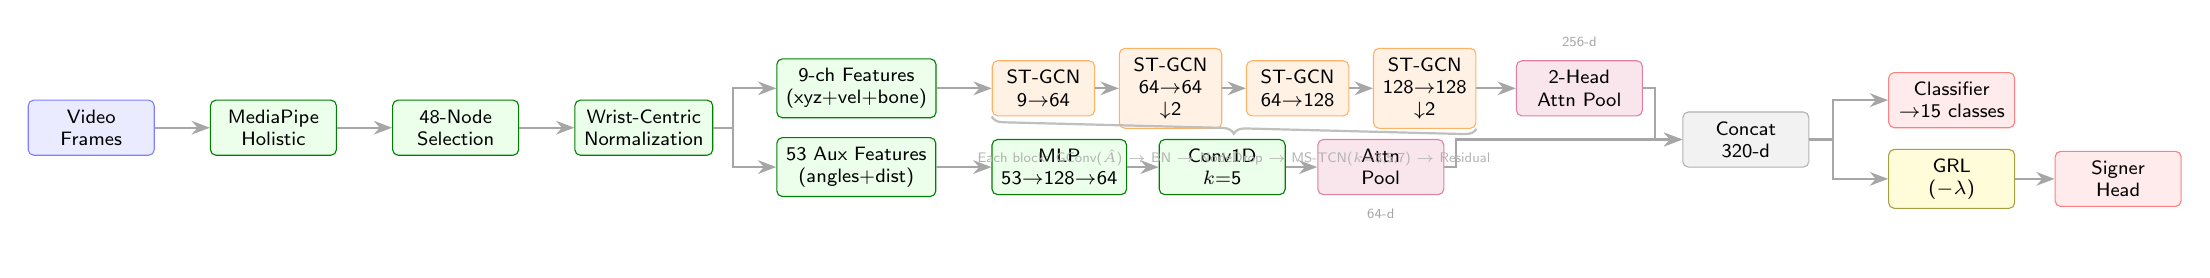
\begin{tikzpicture}[
        node distance=0.5cm and 0.6cm,
        >=Stealth,
        block/.style={rectangle, draw, rounded corners=2pt, minimum height=0.7cm, minimum width=1.6cm, align=center, font=\scriptsize\sffamily},
        input/.style={block, fill=blue!8, draw=blue!50},
        process/.style={block, fill=green!8, draw=green!50!black},
        gcnblock/.style={block, fill=orange!10, draw=orange!60, minimum width=1.3cm},
        pool/.style={block, fill=purple!10, draw=purple!50},
        head/.style={block, fill=red!8, draw=red!50},
        grl/.style={block, fill=yellow!15, draw=yellow!60!black},
        embed/.style={block, fill=gray!10, draw=gray!60},
        arrow/.style={->, thick, draw=gray!70},
        label/.style={font=\tiny\sffamily, text=gray!70},
    ]

    % === INPUT PIPELINE (top row) ===
    \node[input] (video) {Video\\Frames};
    \node[process, right=0.7cm of video] (mp) {MediaPipe\\Holistic};
    \node[process, right=0.7cm of mp] (select) {48-Node\\Selection};
    \node[process, right=0.7cm of select] (norm) {Wrist-Centric\\Normalization};

    % Feature split
    \node[process, right=0.8cm of norm, yshift=0.5cm] (feat9) {9-ch Features\\(xyz+vel+bone)};
    \node[process, right=0.8cm of norm, yshift=-0.5cm] (feat53) {53 Aux Features\\(angles+dist)};

    % === ST-GCN BACKBONE (middle row) ===
    \node[gcnblock, right=0.7cm of feat9] (gcn1) {ST-GCN\\9$\to$64};
    \node[gcnblock, right=0.3cm of gcn1] (gcn2) {ST-GCN\\64$\to$64\\$\downarrow$2};
    \node[gcnblock, right=0.3cm of gcn2] (gcn3) {ST-GCN\\64$\to$128};
    \node[gcnblock, right=0.3cm of gcn3] (gcn4) {ST-GCN\\128$\to$128\\$\downarrow$2};
    \node[pool, right=0.5cm of gcn4] (attn) {2-Head\\Attn Pool};

    % === AUX BRANCH ===
    \node[process, right=0.7cm of feat53] (mlp) {MLP\\53$\to$128$\to$64};
    \node[process, right=0.4cm of mlp] (conv1d) {Conv1D\\$k$=5};
    \node[pool, right=0.4cm of conv1d] (auxpool) {Attn\\Pool};

    % === CONCATENATION ===
    \node[embed, right=0.5cm of attn, yshift=-0.65cm] (concat) {Concat\\320-d};

    % Dimension labels
    \node[label, above=0.05cm of attn] {256-d};
    \node[label, below=0.05cm of auxpool] {64-d};

    % === OUTPUT HEADS ===
    \node[head, right=1.0cm of concat, yshift=0.5cm] (cls) {Classifier\\$\to$15 classes};
    \node[grl, right=1.0cm of concat, yshift=-0.5cm] (grl) {GRL\\($-\lambda$)};
    \node[head, right=0.5cm of grl] (signer) {Signer\\Head};

    % === ARROWS ===
    \draw[arrow] (video) -- (mp);
    \draw[arrow] (mp) -- (select);
    \draw[arrow] (select) -- (norm);
    \draw[arrow] (norm.east) -- ++(0.25,0) |- (feat9.west);
    \draw[arrow] (norm.east) -- ++(0.25,0) |- (feat53.west);

    % GCN chain
    \draw[arrow] (feat9) -- (gcn1);
    \draw[arrow] (gcn1) -- (gcn2);
    \draw[arrow] (gcn2) -- (gcn3);
    \draw[arrow] (gcn3) -- (gcn4);
    \draw[arrow] (gcn4) -- (attn);

    % Aux chain
    \draw[arrow] (feat53) -- (mlp);
    \draw[arrow] (mlp) -- (conv1d);
    \draw[arrow] (conv1d) -- (auxpool);

    % To concat
    \draw[arrow] (attn.east) -- ++(0.15,0) |- (concat.west);
    \draw[arrow] (auxpool.east) -- ++(0.15,0) |- (concat.west);

    % To heads
    \draw[arrow] (concat.east) -- ++(0.3,0) |- (cls.west);
    \draw[arrow] (concat.east) -- ++(0.3,0) |- (grl.west);
    \draw[arrow] (grl) -- (signer);

    % === ST-GCN BLOCK DETAIL (below) ===
    \node[below=1.3cm of gcn2, xshift=0.5cm, font=\scriptsize\sffamily, text=gray!50] (detaillabel) {};

    % Brace under GCN blocks
    \draw[decorate, decoration={brace, amplitude=4pt, mirror}, thick, gray!50]
        (gcn1.south west) -- (gcn4.south east)
        node[midway, below=6pt, font=\tiny\sffamily, text=gray!60, align=center] {Each block: GConv($\hat{A}$) $\to$ BN $\to$ NodeDrop $\to$ MS-TCN($k$=3,5,7) $\to$ Residual};

    \end{tikzpicture}
    \caption{Architecture of the KSL recognition system. Video frames are processed by MediaPipe Holistic to extract 48 skeletal nodes. A 4-layer ST-GCN backbone with multi-scale temporal convolutions processes 9-channel features (joint positions, velocities, bone vectors), while a parallel auxiliary branch captures 53 geometric features (joint angles and fingertip distances). The 320-dimensional combined embedding feeds both a sign classifier and a Gradient Reversal Layer (GRL) that encourages signer-invariant feature learning.}
    \label{fig:architecture}
\end{figure*}

\subsection{Training Strategy}

\subsubsection{Loss Function}
The model trains on a joint loss that combines three objectives:
\begin{equation}
    \mathcal{L} = \mathcal{L}_{\text{CE}} + \alpha \cdot \mathcal{L}_{\text{SupCon}} + \lambda \cdot \mathcal{L}_{\text{signer}}
\end{equation}
where $\mathcal{L}_{\text{CE}}$ is cross-entropy with label smoothing ($\epsilon = 0.1$), $\mathcal{L}_{\text{SupCon}}$ is supervised contrastive loss~\cite{khosla2020supcon} with temperature $\tau = 0.07$ and weight $\alpha = 0.1$, and $\mathcal{L}_{\text{signer}}$ is the adversarial signer classification loss scaled by the GRL schedule $\lambda$.

\subsubsection{Optimization}
We use AdamW with a learning rate of $10^{-3}$ and weight decay $10^{-3}$, paired with cosine annealing ($T_{\max} = 200$, $\eta_{\min} = 10^{-6}$) and a 10-epoch linear warmup. Gradients are clipped at max norm 1.0. Batches of 32, early stopping with patience of 40 epochs, and a signer-balanced batch sampler that cycles through signers within each class to guarantee cross-signer positive pairs for the contrastive loss.

\subsubsection{Mixup and CutMix Regularization}
We apply Mixup~\cite{zhang2018mixup} with $\lambda \sim \text{Beta}(0.2, 0.2)$, blending both GCN and auxiliary inputs with randomly permuted samples and computing loss against both targets. In v25, we added temporal CutMix ($\alpha = 1.0$, applied with probability 0.3) as a mutually exclusive alternative to Mixup: rather than blending two samples smoothly, CutMix splices a contiguous temporal segment from one sample into another, creating more abrupt transitions that we hypothesized would better simulate the variation seen in real-world signing.

\subsubsection{Data Augmentation}
We use 12 augmentation operations applied sequentially during training (Table~\ref{tab:augmentation}). The pipeline went through careful tuning across versions---aggressive augmentations like axis masking got cut after we found they were actually hurting generalization rather than helping it.

\begin{table}[t]
\centering
\caption{Data augmentation pipeline with per-operation probabilities.}
\label{tab:augmentation}
\small
\begin{tabular}{@{}lcc@{}}
\toprule
\textbf{Augmentation} & \textbf{Prob.} & \textbf{Parameters} \\
\midrule
Hand temporal dropout & 0.2 & rate $\sim U(0.1, 0.3)$ \\
Complete hand drop & 0.03 & All frames, one hand \\
Hand swap + X-flip & 0.3 & Swap L/R, negate X \\
Bone-length perturb & 0.5 & scale $\sim U(0.8, 1.2)$ \\
Hand-size scaling & 0.5 & scale $\sim U(0.8, 1.2)$ \\
Z-axis rotation & 0.5 & $\theta \sim U(-15^{\circ}, 15^{\circ})$ \\
Shear transform & 0.3 & shear $\sim U(-0.2, 0.2)$ \\
Joint dropout (spatial) & 0.2 & rate $= 0.08$ \\
Scale jitter & 0.5 & scale $\sim U(0.8, 1.2)$ \\
Spatial noise & 0.4 & $\mathcal{N}(0, 0.015)$ \\
Temporal warp & 0.4 & $\sigma = 0.2$ \\
Temporal shift & 0.3 & shift $\sim U(-8, 8)$ frames \\
\bottomrule
\end{tabular}
\end{table}

\subsection{Evaluation Protocol}

\subsubsection{Validation}
Our validation set has 360 samples per category from a signer held out of training. It gives us a signer-independent evaluation, but one that still shares recording conditions and temporal proximity with training data---so it's optimistic, as we'll see.

\subsubsection{Real-World Testing}
The real test comes from 140 videos (59 numbers, 81 words) recorded by three signers never seen during training or validation. These were shot under naturalistic conditions---varying backgrounds, lighting, signing speeds. This is a strict out-of-distribution evaluation: both the signers and the recording setup differ from anything the model encountered during training.

\subsubsection{Leave-One-Signer-Out Cross-Validation}
In v25, we also ran leave-one-signer-out (LOSO) cross-validation across training signers. Each fold holds out one signer for validation while training on the remaining three, and we average across all folds. This gives a stronger estimate of cross-signer generalization than a single validation split, though as we'll show, even LOSO dramatically overestimates real-world performance.

% ============================================================
% 4. EXPERIMENTS AND RESULTS
% ============================================================
\section{Experiments and Results}

All experiments ran on an NVIDIA A100-PCIE-40GB GPU (MIG 3g.20gb partition) on the Alpine HPC cluster at the University of Colorado Boulder, using PyTorch 2.5.1 with CUDA 12.1.

\subsection{Model Evolution Overview}

Table~\ref{tab:version_summary} traces the progression across seven model versions. Each one introduced specific changes meant to chip away at the generalization gap we kept observing. Some helped. Most didn't.

\begin{table*}[t]
\centering
\caption{Summary of model versions with validation and real-world accuracy. Combined accuracy is weighted by test set size (59 numbers + 81 words = 140 total). Best real-world results are in \textbf{bold}.}
\label{tab:version_summary}
\small
\begin{tabular}{@{}llccccccc@{}}
\toprule
\textbf{Ver.} & \textbf{Key Change} & \textbf{Params} & \textbf{Train} & \textbf{Val} & \textbf{Real} & \textbf{Real} & \textbf{Real} & \textbf{Gap} \\
 & & & \textbf{Time} & \textbf{Comb.} & \textbf{Num.} & \textbf{Words} & \textbf{Comb.} & \textbf{(pp)} \\
\midrule
v19 & Baseline + ArcFace stage 2 & 17.3M & 18.4m & 87.3\% & 20.3\% & 48.1\% & 34.2\% & 53.1 \\
v20 & Aggressive deduplication & 827K & 5.8m & 86.9\% & 18.6\% & 42.0\% & 30.3\% & 56.6 \\
v21 & ArcFace head (full) & 1.47M & 4.6m & 76.5\% & 25.4\% & 37.0\% & 31.2\% & 45.3 \\
v22 & \textbf{No ArcFace, strong GRL} & \textbf{776K} & \textbf{7.3m} & \textbf{93.3\%} & \textbf{33.9\%} & 45.7\% & \textbf{40.7\%} & \textbf{52.6} \\
v23 & 4-stream fusion + focal loss & 3.1M & 35.3m & 95.6\% & 33.9\% & 42.0\% & 38.6\% & 57.0 \\
v24 & Prototypical + MixStyle & 776K & 9.5m & 91.5\% & 25.4\% & 49.4\% & 39.3\% & 52.2 \\
v25 & Hand-body features + CutMix & 777K & 8.2m & 89.1\% & 27.1\% & \textbf{49.4\%} & 38.3\% & 50.8 \\
\bottomrule
\end{tabular}
\end{table*}

\subsection{Best Model Performance (v22)}

Our best overall real-world model turned out to be the simplest one we built after v19. Version 22 strips out ArcFace entirely, cranks up the GRL ($\lambda_{\max} = 0.3$), sticks with a single 9-channel input stream, and uses moderate augmentation. On validation data it hits 91.9\% for numbers and 94.6\% for words (93.3\% combined). On real-world testers: 33.9\% for numbers, 45.7\% for words, 40.7\% combined. That's the best cross-signer generalization we achieved across all seven versions.

It's worth pausing on what that means. We spent considerable effort on versions 23 through 25---multi-stream ensembles, prototypical classification, MixStyle, hand-body features, temporal CutMix---and none of it beat the straightforward single-stream model with a well-tuned GRL.

\subsection{Ablation Studies}

\subsubsection{Test-Time Augmentation}
We initially assumed test-time augmentation would be a free accuracy boost. It wasn't. Table~\ref{tab:tta} shows that TTA---averaging predictions across 5 augmented versions (original, spatial jitter, speed 0.9$\times$, speed 1.1$\times$, and $+5^{\circ}$ rotation)---actually hurts overall accuracy by 1.4 percentage points on v22. Out of 140 predictions, TTA changed only 13, helping 3 (all words) while hurting 5. Average confidence dropped from 0.449 to 0.415. We disabled TTA for all subsequent versions and never looked back. Interestingly, v25 confirmed this finding independently: TTA hurt by 1.2pp there too.

\begin{table}[t]
\centering
\caption{Test-time augmentation impact on v22 real-world accuracy.}
\label{tab:tta}
\small
\begin{tabular}{@{}lccc@{}}
\toprule
\textbf{Method} & \textbf{Numbers} & \textbf{Words} & \textbf{Combined} \\
\midrule
With TTA & 28.8\% & 46.9\% & 39.3\% \\
Without TTA & \textbf{33.9\%} & \textbf{45.7\%} & \textbf{40.7\%} \\
\midrule
Difference & $-5.1$ pp & $+1.2$ pp & $-1.4$ pp \\
\bottomrule
\end{tabular}
\end{table}

\subsubsection{Multi-Stream Fusion (v23)}
Our thinking with v23 was straightforward: if one feature stream is good, four should be better. We trained separate ST-GCN models on joint coordinates, bone vectors, velocity, and bone velocity, then fused them with grid-searched weights and added focal loss for good measure. The validation numbers looked great---95.6\%, the highest we ever saw. But real-world accuracy actually dropped to 38.6\% (Table~\ref{tab:multistream}).

The per-stream breakdown tells the story. The joint stream alone (37.3\% numbers, 42.0\% words) matched or beat the fused result. Stream agreement was dismal: only 18.6\% of number predictions and 29.6\% of word predictions had all four streams agreeing. On in-distribution data, the streams were correlated enough that fusion smoothed out errors. On out-of-distribution data, each stream made different mistakes, and averaging their confusion didn't help.

\begin{table}[t]
\centering
\caption{Per-stream and fused real-world accuracy (v23).}
\label{tab:multistream}
\small
\begin{tabular}{@{}lcc@{}}
\toprule
\textbf{Stream} & \textbf{Numbers} & \textbf{Words} \\
\midrule
Joint & 37.3\% & 42.0\% \\
Bone & 33.9\% & 42.0\% \\
Velocity & 30.5\% & 37.0\% \\
Bone velocity & 35.6\% & 39.5\% \\
\midrule
Fused (4-stream) & 33.9\% & 42.0\% \\
\bottomrule
\end{tabular}
\end{table}

\subsubsection{Prototypical Classification and MixStyle (v24)}
For v24, we swapped the fully-connected classifier for prototypical classification (cosine similarity to class mean embeddings, temperature $\tau = 0.1$) and inserted MixStyle after the first two GCN blocks to synthesize novel signer styles during training. Neither did what we hoped. Prototypical classification reached 25.4\% on numbers and 48.1\% on words (38.6\% combined), while the standard FC head on the same features scored 25.4\% and 49.4\% (39.3\%). Same features, same limitations---the classifier head wasn't the bottleneck.

On the bright side, v24 did achieve the best-ever word accuracy at 49.4\%. But the numbers collapsed to 25.4\%, the worst we'd seen. The two categories seemed to be pulling in opposite directions.

\subsubsection{ArcFace Angular Margin Loss (v21)}
\label{sec:arcface}
Version 21 was, frankly, a disaster. We added ArcFace angular margin loss hoping it would learn more discriminative embeddings. Instead, validation accuracy cratered to 76.5\% and real-world accuracy fell to 31.2\%. The angular margin constraint was simply too aggressive for our tiny signer pool---it collapsed the embedding space rather than sharpening it. We pulled ArcFace entirely for v22 and saw an immediate 16.8pp jump in validation accuracy.

\subsubsection{Hand-Body Spatial Features and Temporal CutMix (v25)}
Version 25 grew out of a diagnostic analysis that revealed something we'd overlooked: our wrist-centric normalization was stripping away hand-to-body spatial information. Many KSL word signs are distinguished partly by \textit{where} the hands are relative to the torso---near the face, at shoulder height, at the waist---and we'd been throwing that signal away.

We added 8 hand-to-body spatial features: hand height relative to shoulder midpoint, lateral hand position relative to shoulders, inter-hand distance (normalized by shoulder width), hand-to-face distance, and a bilateral symmetry measure. We also introduced temporal CutMix ($\alpha = 1.0$, probability 0.3), which splices a contiguous temporal segment from one training sample into another rather than blending them smoothly like Mixup does.

The results were mixed---illuminatingly so. Word accuracy matched the previous best at 49.4\%, but numbers dropped to 27.1\%, and combined accuracy was 38.3\%. What happened? The hand-body features genuinely helped words, where sign location relative to the body carries meaning. But for numbers, which are distinguished primarily by hand shape and finger configuration rather than body position, the extra features just added noise. The model had to learn to ignore them for numbers, and apparently it couldn't do so reliably with only four training signers.

\subsubsection{Leave-One-Signer-Out Cross-Validation (v25)}
To get a more robust estimate of generalization, we ran LOSO cross-validation on v25. Each fold held out one training signer for validation and trained on the other three. The results looked encouraging: 92.4\%$\pm$5.4\% for numbers, 97.1\%$\pm$2.6\% for words, 94.7\% combined.

But here's the problem. Real-world accuracy was 38.3\%. That's a 56.4-point gap between LOSO and the real test. LOSO tells us the model can generalize across the training signers---but those signers share recording conditions, equipment, and temporal context. The three real-world test signers are genuinely out-of-distribution in ways that LOSO can't capture. This is a cautionary result for anyone relying on cross-validation as a proxy for deployment performance in low-resource SLR.

\subsection{Per-Class Analysis}

Table~\ref{tab:perclass_v22} shows per-class accuracy for v22. The variation is dramatic. Three word classes (Friend, Gift, Teach) hit 100\% while four number classes (125, 35, 48, 73) and two word classes (Market, Tomatoes) sit at 0\%. Some classes the model just can't distinguish from others.

\begin{table}[t]
\centering
\caption{Per-class real-world accuracy for v22 (best model). Classes are sorted by accuracy within each category.}
\label{tab:perclass_v22}
\small
\begin{tabular}{@{}lcc|lcc@{}}
\toprule
\multicolumn{3}{c|}{\textbf{Numbers}} & \multicolumn{3}{c}{\textbf{Words}} \\
\textbf{Class} & \textbf{Acc.} & \textbf{n} & \textbf{Class} & \textbf{Acc.} & \textbf{n} \\
\midrule
22 & 75\% & 4 & Friend & 100\% & 6 \\
9 & 75\% & 4 & Gift & 100\% & 4 \\
100 & 50\% & 4 & Teach & 100\% & 6 \\
17 & 50\% & 4 & Tortoise & 83\% & 6 \\
66 & 50\% & 4 & Twin & 67\% & 6 \\
388 & 50\% & 4 & Colour & 50\% & 6 \\
444 & 50\% & 4 & Picture & 50\% & 4 \\
268 & 25\% & 4 & Monday & 33\% & 6 \\
54 & 25\% & 4 & Proud & 33\% & 3 \\
89 & 25\% & 4 & Ugali & 33\% & 6 \\
91 & 25\% & 4 & Agreement & 17\% & 6 \\
125 & 0\% & 4 & Apple & 17\% & 6 \\
35 & 0\% & 3 & Sweater & 17\% & 6 \\
48 & 0\% & 4 & Market & 0\% & 5 \\
73 & 0\% & 4 & Tomatoes & 0\% & 5 \\
\bottomrule
\end{tabular}
\end{table}

The ``sink class'' phenomenon was one of the more puzzling patterns we observed. Certain classes attract a disproportionate number of false predictions---class 66 in v22 numbers (predicted 16 times, actually correct 4 times) and Tortoise in words (predicted 20 times, correct 6 times). These classes seem to sit near the center of the embedding space, catching everything the model isn't sure about.

What's more telling is that the sink class identity keeps changing. Class 66 in v22 became 444 in v23 and v24, then shifted to 91 in v25. Tortoise in v22 became Friend in v24. This instability means the sink phenomenon isn't about specific classes being inherently confusable---it's a side effect of the model latching onto spurious correlations in a small training set.

\subsection{Per-Signer Analysis}

Table~\ref{tab:persigner} breaks down v22 accuracy by test signer. We didn't find a statistically significant signer effect (Cram\'{e}r's V = 0.059 for numbers, $p = 0.90$; V = 0.135 for words, $p = 0.48$), but the individual numbers vary quite a bit, reflecting different signing styles and tempos among our test signers.

\begin{table}[t]
\centering
\caption{Per-signer real-world accuracy for v22 (no-TTA).}
\label{tab:persigner}
\small
\begin{tabular}{@{}lccc@{}}
\toprule
\textbf{Signer} & \textbf{Numbers} & \textbf{Words} & \textbf{n} \\
\midrule
Signer 1 & 31.0\% & 46.4\% & 57 \\
Signer 2 & 33.3\% & 56.0\% & 40 \\
Signer 3 & 40.0\% & 35.7\% & 43 \\
\bottomrule
\end{tabular}
\end{table}

\subsection{Confidence Calibration}

We looked at prediction confidence across versions using the maximum softmax probability, bucketed into HIGH ($>0.6$), MEDIUM ($0.4$--$0.6$), and LOW ($<0.4$). Table~\ref{tab:confidence} shows that calibration varies a lot. In v22, word confidence is well-calibrated---if the model says HIGH for a word, it's right 89\% of the time. But number confidence is badly off: HIGH predictions for numbers are only correct 18\% of the time. The model is confidently wrong on numbers, which is worse than being uncertain.

Version 24's distance-based confidence (sigmoid of the margin between the top-1 and top-2 cosine similarities) did better overall, with HIGH predictions at 79\% accuracy. And v25 was the best calibrated: HIGH at 91\%, MEDIUM at 67\%. So even when v25 didn't improve raw accuracy, it at least knew when to be confident and when not to be.

\begin{table}[t]
\centering
\caption{Accuracy by confidence tier across versions.}
\label{tab:confidence}
\small
\begin{tabular}{@{}llccc@{}}
\toprule
\textbf{Ver.} & \textbf{Category} & \textbf{HIGH} & \textbf{MEDIUM} & \textbf{LOW} \\
\midrule
v22 & Numbers & 18\% & 55\% & 24\% \\
v22 & Words & 89\% & --- & --- \\
v24 & Numbers & 67\% & 21\% & --- \\
v24 & Words & 83\% & 34\% & --- \\
v25 & Combined & 91\% & 67\% & --- \\
\bottomrule
\end{tabular}
\end{table}

\subsection{Top-K Accuracy and Statistical Tests}

For v22, top-2 accuracy hits 57.1\% and top-3 reaches 64.3\% combined. The correct class is usually somewhere in the top few predictions even when it's not the top pick---a useful property for interactive applications where you can show the user a short list of candidates. Cohen's $\kappa$ is 0.236 for numbers and 0.430 for words (fair to moderate agreement), and Matthews Correlation Coefficient (MCC) is 0.245 and 0.446 respectively.

We also ran McNemar's tests comparing v22 against every other version. None of the differences reached statistical significance ($p > 0.05$ across the board). With only 140 test samples, the minimum detectable effect is about 16 percentage points. So while v22 is nominally the best, we can't confidently say it's statistically distinguishable from v24 or v25---all of them are operating in roughly the same performance band, constrained by training data diversity rather than model design.

\subsection{Cross-Version Stability}

Looking at per-class accuracy across versions reveals something troubling: wild instability. A class can go from 75\% in one version to 0\% in the next. Take class 73: 50\% in v19, 0\% in v22, 50\% in v23, 0\% again in v24. Or consider how v25 had 9 of 15 number classes at exactly 0\% accuracy. This kind of volatility, combined with the shifting sink classes, strongly suggests the models are grabbing onto spurious correlations rather than learning genuine sign-discriminative features. With only four training signers, there simply isn't enough variety for the model to figure out what's signer-specific noise and what's actually part of the sign.

\begin{figure}[t]
    \centering
    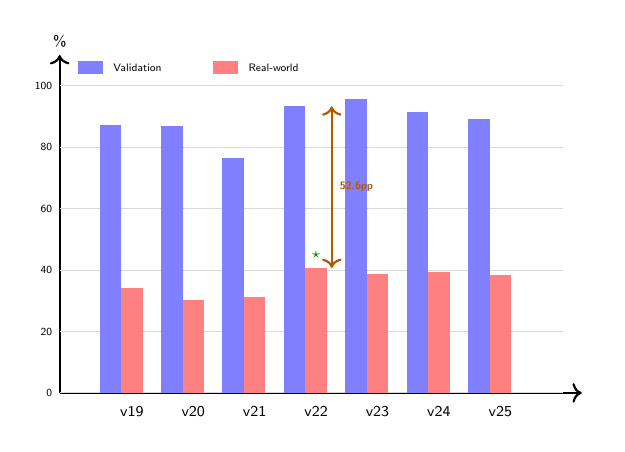
\begin{tikzpicture}[scale=0.78, transform shape]
    \begin{scope}
        % Axes
        \draw[thick, ->] (0,0) -- (8.5,0) node[right, font=\scriptsize\sffamily] {};
        \draw[thick, ->] (0,0) -- (0,5.5) node[above, font=\scriptsize\sffamily] {\%};

        % Y-axis labels
        \foreach \y/\label in {0/0, 1/20, 2/40, 3/60, 4/80, 5/100} {
            \draw[gray!30] (0,\y) -- (8.2,\y);
            \node[left, font=\tiny\sffamily] at (0,\y) {\label};
        }

        % Bar width and positions
        \def\bw{0.35}
        % v19: x=1, v20: x=2, v21: x=3, v22: x=4, v23: x=5, v24: x=6, v25: x=7

        % Validation bars (blue)
        \foreach \x/\val in {1/4.365, 2/4.345, 3/3.825, 4/4.665, 5/4.78, 6/4.575, 7/4.455} {
            \fill[blue!50] (\x-\bw,0) rectangle (\x,\val);
        }

        % Real-world bars (red)
        \foreach \x/\val in {1/1.71, 2/1.515, 3/1.56, 4/2.035, 5/1.93, 6/1.965, 7/1.915} {
            \fill[red!50] (\x,0) rectangle (\x+\bw,\val);
        }

        % Gap arrows for v22 (best)
        \draw[<->, thick, orange!70!black] (4+\bw+0.08, 2.035) -- (4+\bw+0.08, 4.665)
            node[midway, right, font=\tiny\sffamily\bfseries, text=orange!70!black] {52.6pp};

        % X-axis labels
        \foreach \x/\label in {1/v19, 2/v20, 3/v21, 4/v22, 5/v23, 6/v24, 7/v25} {
            \node[below, font=\scriptsize\sffamily] at (\x+\bw/2, -0.1) {\label};
        }

        % Star on v22
        \node[font=\scriptsize, text=green!50!black] at (4+\bw/2, 2.25) {$\star$};

        % Legend
        \fill[blue!50] (0.3, 5.2) rectangle (0.7, 5.4);
        \node[right, font=\tiny\sffamily] at (0.75, 5.3) {Validation};
        \fill[red!50] (2.5, 5.2) rectangle (2.9, 5.4);
        \node[right, font=\tiny\sffamily] at (2.95, 5.3) {Real-world};

    \end{scope}
    \end{tikzpicture}
    \caption{Validation vs.\ real-world combined accuracy across all seven model versions. The gap averages roughly 52.5pp and refuses to close regardless of architecture. Star marks the best real-world model (v22).}
    \label{fig:gap}
\end{figure}

% ============================================================
% 5. DISCUSSION
% ============================================================
\section{Discussion}

\subsection{The Generalization Gap}

The elephant in the room across all seven versions is the persistent chasm between validation and real-world accuracy---averaging about 52.5 percentage points. That's not a typical number in the SLR literature, where most systems get tested on signers who showed up during training, or on large diverse signer pools where the gap is naturally smaller. Our validation set, while held-out by signer, still shares recording equipment, background conditions, and temporal context with the training data. It's a better estimate than testing on training signers, but it's still optimistic.

The gap isn't really about the model. V23 got 95.6\% on validation with four-stream fusion---the model clearly has enough capacity to learn these 30 signs. But real-world accuracy was 38.6\%, actually worse than simpler v22's 40.7\%. More capacity, same ceiling. That pattern---better in-distribution performance paired with flat or declining out-of-distribution performance---is exactly what you'd expect when domain diversity, not model expressiveness, is the bottleneck.

Even LOSO cross-validation, which we added in v25, fell into the same trap. LOSO gave us 94.7\%, which sounds great until you compare it to the 38.3\% real-world number. That's a 56.4-point gap. The training signers, despite being different people, are too similar to each other (same lab, same recording setup, same time period) to meaningfully preview what happens when a genuinely new signer picks up the system.

\subsection{The Four-Signer Ceiling}

Across seven architecturally distinct model versions, real-world accuracy never strayed far from the 30--41\% band, while validation ranged from 76.5\% all the way up to 95.6\%. We believe this is a hard ceiling imposed by having just four unique training signers.

Why? Each signer brings their own quirks---hand shape preferences, speed, movement arc, wrist angles. With four signers, the model can't reliably tease apart what belongs to the signer and what belongs to the sign. The GRL does its best: diagnostic analysis showed signer embedding silhouette scores near zero, meaning the adversarial training successfully scrambled signer identity in the embedding space. But ``not linearly separable by signer'' is a weaker condition than ``genuinely signer-invariant.'' The model may learn features that happen to be signer-invariant across four people but aren't invariant to the broader population of KSL signers.

Multi-stream fusion can't fix this because all streams suffer from the same limited signer diversity. Prototypical classification can't fix it because the prototypes themselves are computed from too few signers. MixStyle can't hallucinate realistic new signers from just four examples. Hand-body features can't fix it because, while they added useful signal for words, they couldn't overcome the fundamental diversity deficit for numbers.

Guo et al.~\cite{guo2024fewshot} got 43.75\% top-1 on ASL with prototypical networks---a result in the same ballpark as ours. That suggests roughly 40\% might be a broader difficulty floor for sign recognition with limited data, not something unique to KSL.

\subsection{What Worked and What Didn't}

Table~\ref{tab:whatworked} is the scorecard. The techniques that actually moved the needle were all about simplification: ripping out ArcFace, tuning the GRL to the right strength, backing off on overly aggressive augmentation, and turning off test-time augmentation. Every ``sophisticated'' addition---multi-stream fusion, prototypical classification, MixStyle, focal loss, post-hoc calibration, hand-body features---either did nothing or made things worse on real-world data.

That last one, hand-body features, is instructive. They demonstrably helped word recognition (where sign location relative to the body matters) but hurt numbers (where hand shape is what counts and body position is just noise). The features weren't bad; they were right for half the problem and wrong for the other half. With more training signers, the model might have learned when to use them and when to ignore them. With four signers, it couldn't.

\begin{table}[t]
\centering
\caption{Summary of techniques explored and their real-world impact.}
\label{tab:whatworked}
\small
\begin{tabular}{@{}lcc@{}}
\toprule
\textbf{Technique} & \textbf{Val Impact} & \textbf{Real Impact} \\
\midrule
Remove ArcFace & $+16.8$ pp & $+9.5$ pp \\
Strong GRL ($\lambda=0.3$) & Neutral & Positive \\
Disable TTA & --- & $+1.4$ pp \\
Moderate augmentation & Positive & Positive \\
\midrule
4-stream fusion & $+2.3$ pp & $-2.1$ pp \\
Focal loss & Neutral & Neutral \\
Post-hoc calibration & Improved & Hurt \\
Prototypical classifier & $-1.8$ pp & $-1.4$ pp \\
MixStyle & Neutral & Neutral \\
Hand-body features & $-4.2$ pp & Words $+$ / Num $-$ \\
Temporal CutMix & Neutral & Neutral \\
ArcFace margin loss & $-16.8$ pp & $-9.5$ pp \\
Aggressive dedup & $-6.4$ pp & $-10.4$ pp \\
\bottomrule
\end{tabular}
\end{table}

\subsection{Numbers vs.\ Words: A Divergence}

One pattern that emerged clearly in the later versions is that numbers and words respond very differently to the same interventions. V24 and v25 both achieved the best-ever word accuracy (49.4\%) while simultaneously producing the worst number results (25.4\% and 27.1\%). Hand-body features helped words but hurt numbers. The two categories apparently rely on different discriminative cues---body-relative location for words, fine-grained hand shape for numbers---and optimizing for one can come at the expense of the other.

This raises a practical question: would it be better to train separate models for numbers and words? We didn't try that here, but it seems like a reasonable next step.

\subsection{Implications for Under-Resourced Sign Languages}

What can other researchers take away from this? A few things.

First, the bottleneck isn't the model. Our best model has 776K parameters and trains in 7 minutes. A model four times larger and five times slower (v23) did worse on real signers. Computational resources aren't the limiting factor.

Second, signer recruitment matters more than architectural sophistication. We tried six different ``clever'' techniques on top of our baseline and none of them broke through the four-signer ceiling. The literature suggests 7--10 signers as a minimum for reasonable cross-signer generalization, and our results are consistent with that.

Third, don't trust your validation accuracy. Our validation numbers ranged from 76\% to 96\%, but real-world performance was always between 30\% and 41\%. Even LOSO, which should be a harder test, overestimated by 56 points. If you're building a system for deployment, test on genuinely new signers.

Fourth, confidence-based rejection can help. V25 showed that when the model was confident (HIGH tier), it was right 91\% of the time. A system that only accepts high-confidence predictions and asks for a re-sign otherwise could be substantially more reliable than raw accuracy suggests.

\subsection{Limitations}

We should be upfront about what this study can't tell you. Our test set is 140 videos from 3 signers---enough to identify the generalization problem, but not large enough for fine-grained statistical comparisons (the minimum detectable effect is about 16 percentage points). The vocabulary covers just 30 isolated signs, while real KSL communication involves hundreds of signs in continuous sequences. We only use manual (hand) features; non-manual markers like facial expressions and head movements carry grammatical meaning in KSL but aren't captured here. The fixed 90-frame window may lose information from unusually long or short signs. And while the model's compact size (776K--777K parameters) and MediaPipe's real-time capability suggest deployment is feasible, we haven't benchmarked inference latency in a production setting.

% ============================================================
% 6. CONCLUSION
% ============================================================
\section{Conclusion}

We built the first automated Kenya Sign Language recognition system and, over seven iterations, learned more from our failures than our successes. The best model (v22)---a compact ST-GCN with gradient reversal---gets 93.3\% on validation but only 40.7\% on unseen signers. That gap held steady across seven architecturally diverse versions, through multi-stream fusion, prototypical classification, MixStyle, hand-body features, and temporal CutMix. LOSO cross-validation painted an equally misleading picture at 94.7\% versus 38.3\% real-world.

The conclusion we keep arriving at is simple, even if it's not the one we wanted: the generalization barrier here is fundamentally about data diversity, not model design. Four training signers aren't enough, and no architectural trick we tried could make them enough. This is a negative result in some sense, but we think it's a valuable one. For anyone building SLR systems for under-resourced sign languages, the message is clear: recruit more signers before you reach for a bigger model.

That said, the system isn't without promise. V25's confidence calibration shows that when the model knows what it's looking at, it's usually right (91\% at the HIGH tier). A deployment that selectively accepts high-confidence predictions could be genuinely useful even at current accuracy levels. And the hand-body features, while they didn't improve overall accuracy, did push word recognition to its best result (49.4\%), suggesting that the feature representation itself has room to grow once more signer diversity is available.

Going forward, the path is straightforward: expand to 7--10 signers, extend the vocabulary to continuous signing, add non-manual markers, and revisit techniques like hand-body features and CutMix that showed partial promise. We release our code and evaluation protocol so others can build on this work.

% ============================================================
% REFERENCES
% ============================================================
\bibliographystyle{IEEEtran}

\begin{thebibliography}{24}

\bibitem{ai4ksl2024}
AI4KSL Project, ``Creating a digital open-access Kenya Sign Language dataset,'' \textit{arXiv preprint arXiv:2410.18295}, 2024.

\bibitem{aiman2023}
U.~Aiman and T.~Ahmad, ``Angle based hand gesture recognition using graph convolutional network,'' \textit{Computer Animation and Virtual Worlds}, vol.~35, no.~1, 2023.

\bibitem{amukasa2021}
Amukasa, ``Translating the Kenyan Sign Language with Deep Learning,'' Technical report, 2021.

\bibitem{anithadevi2025}
N.~Anithadevi \textit{et al.}, ``MediaPipe-LSTM-Enhanced Framework for Real-Time Dynamic Sign Language Recognition in Inclusive Communication Systems,'' \textit{Engineering Reports}, vol.~7, no.~7, 2025.

\bibitem{chen2021ctrgcn}
Y.~Chen \textit{et al.}, ``Channel-wise Topology Refinement Graph Convolution for Skeleton-Based Action Recognition,'' in \textit{Proc. ICCV}, 2021.

\bibitem{deng2019arcface}
J.~Deng \textit{et al.}, ``ArcFace: Additive Angular Margin Loss for Deep Face Recognition,'' in \textit{Proc. CVPR}, 2019.

\bibitem{ganin2016domain}
Y.~Ganin \textit{et al.}, ``Domain-Adversarial Training of Neural Networks,'' \textit{J. Machine Learning Research}, vol.~17, no.~59, pp.~1--35, 2016.

\bibitem{guo2024fewshot}
Guo \textit{et al.}, ``Data-Efficient American Sign Language Recognition via Few-Shot Prototypical Networks,'' \textit{arXiv preprint arXiv:2512.10562}, 2024.

\bibitem{hasan2025}
A.~Hasan \textit{et al.}, ``Bangla Sign Language Recognition With Multimodal Deep Learning Fusion,'' \textit{Engineering Reports}, vol.~7, no.~4, 2025.

\bibitem{kamal2024}
S.~M.~Kamal \textit{et al.}, ``Adversarial autoencoder for continuous sign language recognition,'' \textit{Concurrency and Computation: Practice and Experience}, vol.~36, no.~22, 2024.

\bibitem{khosla2020supcon}
P.~Khosla \textit{et al.}, ``Supervised Contrastive Learning,'' in \textit{Proc. NeurIPS}, 2020.

\bibitem{kolawole2024augmentation}
Kolawole \textit{et al.}, ``Enhancing Human Action Recognition with 3D Skeleton Data: A Comprehensive Study of Deep Learning and Data Augmentation,'' \textit{Electronics}, vol.~13, no.~4, p.~747, 2024.

\bibitem{liu2020msg3d}
Z.~Liu \textit{et al.}, ``Disentangling and Unifying Graph Convolutions for Skeleton-Based Action Recognition,'' in \textit{Proc. CVPR (Oral)}, 2020.

\bibitem{moustafa2023}
A.~M.~Moustafa \textit{et al.}, ``Integrated Mediapipe with a CNN Model for Arabic Sign Language Recognition,'' \textit{J. Electrical and Computer Engineering}, 2023.

\bibitem{pu2024signer}
J.~Pu \textit{et al.}, ``Improving Continuous Sign Language Recognition with Consistency Constraints and Signer Removal,'' \textit{ACM Trans. Multimedia Computing, Communications, and Applications}, 2024.

\bibitem{robert2023review}
E.~J.~Robert and H.~J.~Duraisamy, ``A review on computational methods based automated sign language recognition system,'' \textit{Concurrency and Computation: Practice and Experience}, vol.~35, no.~9, 2023.

\bibitem{shi2019twostreamAGCN}
L.~Shi \textit{et al.}, ``Two-Stream Adaptive Graph Convolutional Networks for Skeleton-Based Action Recognition,'' in \textit{Proc. CVPR}, 2019.

\bibitem{snell2017prototypical}
J.~Snell \textit{et al.}, ``Prototypical Networks for Few-shot Learning,'' in \textit{Proc. NeurIPS}, 2017.

\bibitem{yan2018stgcn}
S.~Yan \textit{et al.}, ``Spatial Temporal Graph Convolutional Networks for Skeleton-Based Action Recognition,'' in \textit{Proc. AAAI}, 2018.

\bibitem{zhang2018mixup}
H.~Zhang \textit{et al.}, ``mixup: Beyond Empirical Risk Minimization,'' in \textit{Proc. ICLR}, 2018.

\bibitem{zhang2020mediapipe}
F.~Zhang \textit{et al.}, ``MediaPipe Hands: On-device Real-time Hand Tracking,'' \textit{arXiv preprint arXiv:2006.10214}, 2020.

\bibitem{zhou2021mixstyle}
K.~Zhou \textit{et al.}, ``Domain Generalization with MixStyle,'' in \textit{Proc. ICLR}, 2021.

\end{thebibliography}

\end{document}
